\documentclass{article}
% ============= Page size margins etc.
% ============= This offers great flexibility in terms of document size
\usepackage{geometry}
\geometry{twoside,
          letterpaper, % i.e, paperwidth=210mm and paperheight=297mm,
          top=25mm,
          bottom=40mm,
          left=25mm,
          right=25mm,
}
% =========== Math related stuff
% There are more tools for handling fractions etc.
% but can be left out until the need is obvious
\usepackage{mathtools} %<- Fixes, enhances amsmath package (loads amsmath too so no need to load it)
\usepackage{amssymb,amsthm}% Standard AMS tools

% =========== Graphics-related stuff
\usepackage{graphicx} % don't load epsfig or psfig
\usepackage[colorlinks = true,
            linkcolor = blue,
            urlcolor  = blue,
            citecolor = blue,
            anchorcolor = blue]{hyperref}

\usepackage{xcolor}


%Let's replicate the handout for demo, I'll call mytitle
\newcommand{\myTitleBox}{
\noindent\makebox[\linewidth][c]{%
  \colorbox{gray!30}{%
    \parbox{\paperwidth}{%
      \hspace*{\dimexpr\hoffset+\oddsidemargin+1in\relax}%
      \begin{minipage}{\dimexpr\textwidth-2\fboxsep-2\fboxrule\relax}
      {\large\textbf{\courseTitleS}\courseTitle\hfill}\vspace{2mm}\\
      {\large\textbf{\topicsCoveredS}\topicsCovered\hfill}\vspace{2mm}\\
      {\large\courseInstructors\hfill}\vspace{2mm}\\
      \secAuthor\hfill\sectionTimesV\\
      \authorContact\hfill\sectionTime\\
      \end{minipage}
    }%
  }%
}
}

\setlength{\parskip}{1em}
\setlength{\parindent}{0pt}

\newcommand{\courseTitleS}{CS109A/STAT121A/APCOMP209a:}
\newcommand{\courseTitle}{ Introduction to Data Science}
\newcommand{\courseInstructors}{\textbf{Instructors:} Pavlos Protopapas, Kevin Rader}
\newcommand{\sectionTimesV}{Section Times}
\newcommand{\sectionTime}{ Wed 3-4pm \& Wed 5:30-6:30 \& Thurs 2:30-3:30}
\newcommand{\topicsCoveredS}{Advanced Section 6:}
\newcommand{\topicsCovered}{ Topics in Supervised Classification}
\newcommand{\authorContact}{nhoernle@g.harvard.edu}
\newcommand{\secAuthor}{Nick Hoernle}
\newcommand{\emptyS}{ }


\author{Nick Hoernle}



\begin{document}
\myTitleBox

\section{Classification Recap}
%During the `hypothesis testing' section of Linear Regression, we saw a philosophy of reasoning where scientists present hypotheses, detail the assumptions that were made in presenting the hypotheses, and then evaluate the probability of observing the sampled data under those hypotheses. We have further seen that while certain  hypotheses can be rejected (as highly improbable), it is difficult to simply `accept' the alternative upon `rejecting' the null. In contrast to this approach, Bayesian statistics is concerned with evaluating the plausibility of an event given incomplete knowledge. In other words, instead of falsifying hypotheses using statistical tests, we rather employ an inductive approach of learning about general systems via the specific observations at hand and the beliefs of the scientist before obtaining the observed data \cite{gelman2013philosophy}.
% There are two competing schools of thought in Statistics which present different perspectives on the problem of understanding model parameters given a set of observed data. \textit{Frequentist} reasoning dictates that a true process (with fixed parameters) generates a population of data, and for this discussion we can assume that the population is infinite. The specific sample that we then obtained is a small sample of data from that population and thus there is stochasticity involved in the conclusions that we can draw becuase of the sampled nature of this data. Specifically, we evaluate the probability that another random sample of data would present model parameters that are similar to the ones that we have observed.
% During the `hypothesis testing' section of Linear Regression, we saw a philosophy of reasoning where we were presented with a sample from a `true' underlying statistical process. This sample represented a subset of data from the truth
% [PP: truth, shall we use population?]
% and we used hypothesis testing to evaluate the probability of the true parameters being different from a specific null hypothesis, given the noisy and incomplete data. The specific observed data was the result of a random sampling procedure from a set of complete data (that would describe the model in its entirety).
% \textit{Bayesian} statistics takes a contrasting approach that dictates there is a distribution over the values that the parameters can hold given the fixed sample of data that we have observed. In this case, we consider the sample of data as fixed and rather try to understand what the specific sample implies for the probability of having a certain model.

% [PP: I like this, but I would emphasize that in frequentist there is a "truth" model and data are noisy and incomplete, where in Bayesian statistics model (parameters) have a distribution. It is all there as you described. I would have switch the order a little.First mention the sample data but true model, then hypothesis testing and then  mention bayesian. Also, it may be best not mention hypothesis testing as add on to freq. approach. ]

% the sampling is no longer the random process but the actual system itself is a stochastic model. Considering the problem this way allows Bayesian data scientists to concern themselves with evaluating the plausibility of an event given incomplete knowledge.

% In other words they employ an inductive approach of learning about general systems via the specific observations at hand and the beliefs of the scientist before obtaining the observed data \cite{gelman2013philosophy}.

 % scientists present hypotheses, detail the assumptions that were made in presenting the hypotheses, and then evaluate the probability of observing the sampled data under those hypotheses. We have further seen that while certain  hypotheses can be rejected (as highly improbable), it is difficult to simply `accept' the alternative upon `rejecting' the null. In contrast to this approach, Bayesian statistics is concerned with evaluating the plausibility of an event given incomplete knowledge. In other words, instead of falsifying hypotheses using statistical tests, we rather employ an inductive approach of learning about general systems via the specific observations at hand and the beliefs of the scientist before obtaining the observed data \cite{gelman2013philosophy}.

 We have already seen a popular way of making a classification decision between two classes by evaluating the \textit{log-odds} that a datapoint belongs to one or the other class. Under the assumption that the log-odds ratio is linear in the predictors, we arrived at Logistic Regression. Linear Discriminant Analysis presents another technique for finding a linear separating hyperplane between two classes of data. Consider a problem where we have data drawn from two multivariate Gaussian distributions: $X_1 \sim N(\mu_1, \Sigma_1)$ and $X_2 \sim N(\mu_2, \Sigma_2)$. If we wish to make a classification decision for a new datapoint, we can evaluate the probability that the datapoint belongs to a class and can again study the ratio of these probabilities to make that decision.

Since, we are interested in evaluating the probability that a datapoint belongs to a certain class, we wish to evaluate: $p(Y=k \vert X = x)$ (i.e. given datapoint x, what is the the probability that it belongs to class k). Using the axioms of probability (and specifically those of conditional probability), we can derive Bayes rule:
$$
p(Y=k|X=x) = \frac{p(X=x, Y=k)}{p(X=x)} = \frac{p(X=x|Y=k)p(Y=k)}{p(X=x)}
$$

This probability is often termed the \textit{posterior distribution}. The joint probability ($p(x, y)$) mass or density function can be factored into a multiplication of the \textit{prior distribution} $p(y)$ and the \textit{sampling distribution} or \textit{likelihood function} $p(x \vert y)$. Bayes' rule expresses the \textit{posterior} density in terms of the \textit{prior}, the \textit{likelihood} and the \textit{evidence or marginal likelihood} $p(x)$ \cite{gelman2013philosophy} \cite{gelman2014bayesian}. For simplification of notation, if we let $f_k(x)$ denote the class-conditional density of $x$ in the class $Y=k$, and we let $\pi_k$ be the \textit{prior probability} that a datapoint chosen at random will be observed as class k (note that $\sum_{k=1}^K \pi_k = 1$), we obtain:

$$
p(Y=k|x) = \frac{f_k(x) \pi_k}{\sum_{l=1}^K f_l(x) \pi_l}
$$

% [PP: posterior distribution is not defined]
% $$
% p(Y=k|X=x) = \frac{p(X=x|Y=k)p(Y=k)}{p(X=x)} = \frac{f_k(x) \pi_k}{\sum_{l=1}^K f_l(x) \pi_l}
% $$
% [PP: move the footnote out of the equation]

% When the sampling distribution is considered a function of $\theta$ for a fixed $y$ (which in the Bayesian framework is the case) it called the \textit{likelihood function}.
% [PP: eh? why so complicated? WHy not calling it liklihood from the beginning?]

% When optimising $p(y \vert \theta)p(\theta)$ (a function of $\theta$), it is common to ignore an often intractable $p(y)$ (constant with respect to the optimisation over $\theta$) and thus the simpler $p(\theta \vert y) \propto p(y \vert \theta)p(\theta)$ is used. From this relationship, the data $y$ can be seen to affect the posterior density only through $p(y \vert \theta)$ \cite{gelman2014bayesian}. When this quantity is considered a function of $\theta$ for a fixed $y$ (which in the Bayesian framework is the case) we give a different name to the \textit{sampling distribution} and call it the \textit{likelihood function}.

In logistic regression, you actually already reasoned about the best classification decision using the \textit{posterior} probability that a classification should be a $0$ or a $1$. In that case, we evaluated the \textit{log-odds} for the classification decision of one class over another. From what was discussed in class, minimising the misclassification rate corresponds to maximising the posterior probability that a datapoint should be classified to class $k$. Making a classification decision by maximising the posterior probability results in a \textit{Bayes' classifier} (note that choosing a decision boundary is a field of study in it own rights and is known as Decision Theory).


\section{Linear Discriminant Analysis (LDA)}\label{sec:lda}
LDA makes the explicit assumption that for each of the $K$ classes, the class conditional densities $p(x|Y=k) = f_k(x)$ are multivariate Gaussian distributions. We therefore have $P(x|Y=k) \sim N(\mu_k, \Sigma_k)$ which means that the densities follow:

$$
f_k(x) = \frac{1}{(2\pi)^{p/2} \vert \Sigma_k \vert ^{1/2} } \exp \big \{\frac{-1}{2}(x - \mu_k)^T \Sigma_k^{-1} (x - \mu_k) \big \}
$$

If this is the case, we wish to analyse the posterior probability that an unlabeled datapoint belongs to one of the classes and select the class that maximises this posterior probability (i.e. classify the datapoint to the class $k$ that maximises $p(Y=k \vert x)$). Thinking about the two class classification problem is illuminating. If we have $f_1(x)$ and $f_2(x)$ as the multivariate Gaussian distributions for classes $1$ and $2$ respectively with prior probabilities $\pi_1$ and $\pi_2$, we would classify the datapoint $x$ to $\arg\max\limits_k(p(Y=k \vert x)) = \arg\max\limits_k(\log p(Y=k \vert x))$. We can now apply Bayes' rule and drop the denominator that is independent of k to rather find the class $k$ which $\arg\max\limits_k(\log(\pi_k) + \log(f_k(x)))$. We therefore obtain the following discriminant function ($\delta_k(x)$) for each class $k$ remembering that we select k with the highest $\delta_k(x)$, (noting again that the common $2\pi$ constant can also be dropped from the maximisation):

$$
\delta_k(x) = log(\pi_k) - \frac{1}{2}log(\vert \Sigma_k \vert) - \frac{1}{2}(x - \mu_k)^T \Sigma_k^{-1} (x - \mu_k)
$$

It is worth noting that $(x - \mu_k)^T \Sigma^{-1}_k (x - \mu_k)$ is known as the (squared) Mahalanobis distance metric and it is a measure of the distance between a point and a distribution. LDA further makes the assumption that the covariance matrices of the different classes are equal: $\Sigma_1 = \Sigma_2 = \dots = \Sigma_k = \Sigma$. We can analyse the \textit{decision boundary} between two classes where the discriminant functions are exactly equal:

\begin{align*}
\delta_1(x) &= \delta_2(x) \\
log(\pi_1) - \frac{1}{2}log(\vert \Sigma \vert) - \frac{1}{2}(x - \mu_1)^T \Sigma^{-1} (x - \mu_1) &= log(\pi_2) - \frac{1}{2}log(\vert \Sigma \vert) - \frac{1}{2}(x - \mu_2)^T \Sigma^{-1} (x - \mu_2) \\
0 &= log(\frac{\pi_1}{\pi_2}) - \frac{1}{2}(\mu_1 + \mu_2)^T \Sigma^{-1}(\mu_1 - \mu_2) + x^T\Sigma^{-1}(\mu_1 - \mu_2)
\end{align*}

This result is linear in $x$ and it discriminates between the data from class 1 and the data from class 2 (hence the `linear discriminant' analysis). Notice that the $x^T \Sigma x$ term is canceled out (as again this term is independent of $k$ and therefore does not play a role in the maximisation).


\section{Quadratic Discriminant Analysis}

The setup for this problem is exactly the same, but here we relax the pooled variance assumption and rather allow the individual classes to have their own class specific covariances. We therefore still arrive at the same discriminant function as before:

$$
\delta_k(x) = log(\pi_k) - \frac{1}{2}log(\vert \Sigma_k \vert) - \frac{1}{2}(x - \mu_k)^T \Sigma_k^{-1} (x - \mu_k)
$$

But when evaluating the decision boundary between the classes, the algebra becomes a little messy in deriving the result \footnote{You should validate this result yourselves for practice}:

\begin{equation*}
0 = log(\frac{\pi_1}{\pi_2}) + \frac{1}{2}log(\frac{\vert \Sigma_2 \vert}{\vert \Sigma_1 \vert}) - \frac{1}{2} \big[ \mu_1^T \Sigma_1^{-1} \mu_1 - \mu_2^T \Sigma_2^{-1} \mu_2 + 2 x^T (\Sigma_2^{-1}\mu_2 - \Sigma_1^{-1}\mu_1)  + x^T (\Sigma_1^{-1} - \Sigma_2^{-1}) x \big]
\end{equation*}

The $x^T (\Sigma_1^{-1} - \Sigma_2^{-1}) x$ term now shows that this decision boundary is quadratic in $x$.

%  Further note that for the two class problem (with class 1 and class 2), $\delta_1(x) = \delta_2(x)$ represents the decision boundary between the two classes, and this decision boundary is quadratic in $x$ (\textit{refer to your lecture notes for more on this topic}).
%
% Dealing with the case that the classes have the same (pooled) covariance matrices, we have the objective of classifying the datapoint to the class that maximises:
% $$
% \delta_k(x) = x^T \Sigma^{-1}\mu_k + log(\pi_k) -\frac{1}{2}\mu_k^T\Sigma^{-1}\mu_k
% $$
%
% [PP: We can demonstrate that for 1-d this gives the same results as above]
% [PP: This is linear in x]

% [PP: The term x Sigma x disappears. Why? Because it is indep of k ]

% Again, for the two class problem, we can look at the log posterior-odds:
% $$
% \frac{p(Y=k \vert X=x)}{p(Y=l \vert X=x)} = \frac{f_k(x)\pi_k}{f_l(x)\pi_l} = log\frac{\pi_k}{\pi_l} - \frac{1}{2}(\mu_k+\mu_l)^T\Sigma^{-1}(\mu_k-\mu_l) + x^T \Sigma^{-1}(\mu_k - \mu_l)
% $$
% Note now that the decision boundary would be linear in $x$. Further note that the $\Sigma^{-1}(\mu_k - \mu_l)$ direction term is the same as the $\mathbf{w}$ vector found above.

\section{Fisher's Linear Discriminant}

In \href{https://github.com/cs109/a-2017/blob/master/Sections/advanced/sec4.pdf}{Section 4} we discussed the dimensionality reduction method of Principal Component Analysis (PCA). Similarly, LDA can be thought of as a dimensionality reduction technique where a linear discriminant is found that attempts to maximally separate two different classes. PCA, under its assumptions, attempts to find the Principal Components that account for most of the variance in the dataset. On the other hand, LDA attempts to model the difference between the classes of data.\footnote{It is worth noting LDA is a supervised technique whereas PCA is unsupervised even though, in this case, we are comparing them for the same function of dimensionality reduction.}

% [PP: Actually this is a point I have been making in OH. PCA does not look at Y at all so it is not guaranteed to help with classification or regression. I think this statement is true. It just reduces the dimensionality, reduces overfitting but I think in principle model selection must be far superior. Let's talk about it more]

Let's imagine an example in two dimensions with data belonging to one of two classes, where the two classes have (Gaussian) marginal distributions that are highly elongated but aligned (see figure \ref{fig:lda_vs_pcs_ex} for an example).
\begin{figure}[h]
\center
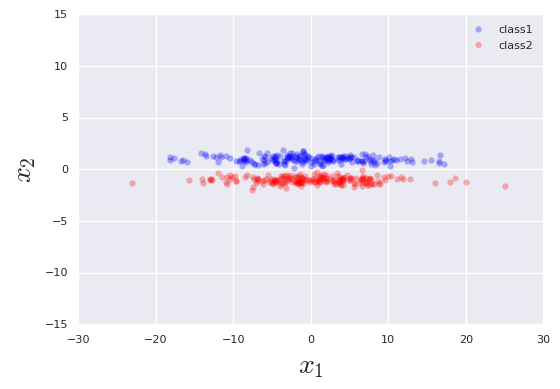
\includegraphics[width=8cm]{lda_vs_pcs_ex}
\caption{Example dataset where LDA will present a more useful dimensionality reduction than PCA}\label{fig:lda_vs_pcs_ex}
\end{figure}
As you learned, the first principal component will extract the dimension that captures the highest variance in the data (in this case it will be exactly $x_1$). For the purposes of dimensionality reduction, projecting the data onto this component will result in a one dimensional representation where the data is entirely inseparable (see figure \ref{fig:pca_projection}).\footnote{For the purposes of visualising the data, I have added a small amount of vertical jitter for plotting the points.}

\begin{figure}[h]
\center
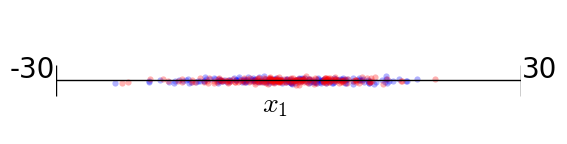
\includegraphics[width=8cm]{pca_projection}
\caption{Example of a projection that does not discriminate between the data classes}\label{fig:pca_projection}
\end{figure}

We can clearly see that for the task of classification, a more useful projection would be one onto the $x_2$ component. Fisher Linear Discriminant Analysis (LDA) considers maximising an objective with the goal of finding a \textit{discriminating} hyperplane between these classes \cite{welling2005fisher} (and not the hyperplane that describes the variance of the dataset in its entirety). LDA uses the additional information of known class labels to find a more useful discriminator between the data classes.

Classification in a high dimensional space is hard as the relevative distances between data becomes extremely sparse making distance metrics less useful. This is known as the curse of dimensionality \cite{parsons2004subspace}. Rather, imagine we were able to perform a projection of the data onto a lower dimensional subspace, such that the means of the data clusters are maximally separated, yet the variances of the within cluser data are minimised. LDA actually performs this projection (under the assumption of Gaussian data).

Let $\mathbf{W}$ be a matrix that consists of column vectors $\mathbf{w}$ that each represent a hyperplane that discriminates between two classes. Our aim is to find $\mathbf{W}$ such that the objective of maximising the distances between the means of the classes and minimising the within class variance is achieved. To do this, we need the \textit{between-class scatter} matrix (measuring the spread of the class means)

$$S_B = \sum_k(\mathbf{\mu_k - \mathbf{\bar{x}}})(\mathbf{\mu_k - \mathbf{\bar{x}}})^T$$

where $\mu_k$ is the mean of class $k$ and $\bar{X}$ is the mean of the entire dataset. And we need the \textit{total within-class scatter} matrix

$$S_W = \sum_k \sum_{i \in k}(\mathbf{x_i} - \mathbf{\mu_k})(\mathbf{x_i} - \mathbf{\mu_k})^T$$

there are $K$ classes, with $k = \{1, \dots, K\}$ indexing the $k^{th}$ class and $i \in k$ means that observation $i$ is in class $k$; thus $x_i$ is a datapoint in class $k$. The optimisation task is then to find the vector $\mathbf{w}$ that maximises the following objective (also called the Rayleigh quotient):

$$
J(\mathbf{w}) = \frac{\textrm{between class scatter}}{\textrm{within class scatter}} = \frac{\mathbf{w}^TS_B\mathbf{w}}{\mathbf{w}^TS_W\mathbf{w}}
$$

Again, it is helpful to study the two class case: let's assume we have data from two Gaussian distributions $(X|Y=1) \sim N(\mu_1, \Sigma_1$) and $(X|Y=2) \sim N(\mu_2, \Sigma_2$) for classes $1$ and $2$ respectively. We have $S_B = \sum\limits_{k=1}^2(\mathbf{\mu_k - \mathbf{\bar{x}}})(\mathbf{\mu_k - \mathbf{\bar{x}}})^T = (\mu_1 - \mu_2)(\mu_1 - \mu_2)^T$ and $S_W = (\Sigma_1 + \Sigma_2)$.
% [PP: I do not see the  $S_B = (\mu_1 - \mu_2)(\mu_1 - \mu_2)^T$ ! What is $\bar{x}$?] - this is just an application of the bias - variance expansion

Maximising the objective $J$ with respect to $\mathbf{w}$ is equivalent to maximising the numerator while holding the denominator constant as both the numerator and denominator have the same order of $\Vert\mathbf{w}\Vert$ and thus J is invariant to scale changes in $\Vert\mathbf{w}\Vert$. Further, as we are only interested in the direction of $\mathbf{w}$, we can hold the denominator constant to $1$. So we find $\mathbf{w}$ to $max (\mathbf{w}^TS_B\mathbf{w})$ such that $\mathbf{w}^TS_W\mathbf{w} = 1$ which results in the following Legrangian:

$$
L = \mathbf{w}^T S_B\mathbf{w} + \lambda(\mathbf{w}^T S_W\mathbf{w} - 1)
$$

Setting $\frac{\partial L}{\partial \mathbf{w}}$ to $0$ yields $2(S_B - \lambda S_W)\mathbf{w} = 0$ and so:

\begin{equation*}
  S_W^{-1}S_B \mathbf{w} = \lambda \mathbf{w}
\end{equation*}

In general the solution exists if $S_W^{-1}$ exists. Moreover, the solution is not unique and corresponds to the eigenvalue problem for the $S_W^{-1}S_B$ matrix.

Referring back to the two class case, and using the definition of $S_B$ in the two class case, we see that
\begin{equation*}
S_W^{-1}S_B \mathbf{w} = S_W^{-1}(\mu_1 - \mu_2)(\mu_1 - \mu_2)^T \mathbf{w} = \lambda \mathbf{w}
\end{equation*}

and finally noting that $(\mu_1 - \mu_2)^T \mathbf{w} = \alpha$ is a scalar we get:
\begin{equation*}
  S_W^{-1} (\mu_1 - \mu_2) = \frac{\lambda}{\alpha} \mathbf{w}
\end{equation*}
% [PP: I guess $\alpha = (\mu_1 - \mu_2)^T \mathbf{w}$. ]

% [PP: why is it a scalar? Not obvious to me. Even if it a scalar it depends on the values of w, but I guess we are only interested in the direction]

Again, we are only interested in the direction of $\mathbf{w}$ (and can discard the scalar multiplier), so
\begin{equation}
\mathbf{w^*} = S_W^{-1} (\mu_1 - \mu_2)
\end{equation}

If you refer back to Section \ref{sec:lda} you should see that $S_W^{-1} (\mu_1 - \mu_2) = 2\Sigma^{-1} (\mu_1 - \mu_2)$ gives the same direction vector for the decision boundary that was found in that Section.

In the more general case where we have $K$ classes (and $K$ associated means $\mu_k$), with $K \geq 2$, LDA constructs a $\mathbf{W}$ matrix that spans a maximum of $K-1$ dimensions. Moreover, when the data are in $\mathcal{R}^P$, with $P > K$, LDA can be seen as a method that projects the $P$ dimensional data onto a $K-1$ dimensional subspace for which the data is maximally (linearly) separated into its clusters.

% [PP: Which space? Are we talking the w-dim? WHY?]

You can reach this result by studying the rank of the $S_W^{-1}S_B$ matrix. We firstly need the result\cite{petersen2008matrix} that:
\begin{equation}\label{eq:rankmin}
  rank(S_W^{-1}S_B) \leq \min\{ rank(S_W^{-1}), rank(S_B) \}
\end{equation}

Secondly, \textbf{Lemma 1:} $rank(S_B) \leq K-1$.

\textbf{Proof:} Consider $P$ dimensional multivariate vectors $\mu_k$ with $k = 1 \hdots K$ drawn i.i.d from a distribution with mean $\mathbf{\bar{x}}$. The covariance matrix can be estimated by the drawn samples:
$$
\hat{Var(\mu)} = \frac{1}{K} \sum\limits_{k=1}^K (\mu_k-\mathbf{\bar{x}})(\mu_k-\mathbf{\bar{x}})^T
$$
Interpreting this result as a covariace matrix is noting that the estimate must have K-1 degrees of freedom. Now, note that $S_B = K\hat{Var(\mu)}$. Recall again that an assumption is that $K$, the number of classes, is less than $P$, the number of dimensions, and therefore $S_B$ is not a full rank matrix. It follows that $S_B$ also has $K-1$ degrees of freedom corresponding to $rank(S_B) \leq K-1$.


Finally, since $rank(S_B) \leq K-1$ and from eq \ref{eq:rankmin}, we see that the rank of $S_W^{-1}S_B$ is less than or equal to $K-1$. A last note on the dimensionality reduction is that if $P$, the number of dimensions, is greater than $K$, the number of classes, then $S_B$ is full rank with $rank(S_B) = P$ and thus LDA results in no dimensionality reduction.
% he result that $S_W^{-1}S_B$ is of rank $K-1$
% $S_B = \sum_k(\mu_k - \mathbf{\bar{x}})(\mu_k - \mathbf{\bar{x}})^T$

% $rank(S_B) \leq K-1$ as $S_B$ is the sum of $K$ matrices that have rank one or less.} So LDA projects a p dimensional vector onto a $K-1$ dimensional subspace for which the data is maximally (linearly) separated.

% and we consider the space that is spanned by the mean vectors for each of the classes, these vectors only span a space of $K-1$ dimensions. it can be shown that $S_W^{-1}S_B$ is of rank $K-1$.

% Where $S_B = \sum_k(\mathbf{\mu_k - \mathbf{\bar{x}}})(\mathbf{\mu_k - \mathbf{\bar{x}}})^T$ and $S_W = \sum_k \sum_{i \in k}(\mathbf{x_i} - \mathbf{\mu_k})(\mathbf{x_i} - \mathbf{\mu_k})^T$. I.e. $S_B$ is the scatter matrix between the cluster means (\textit{between-class scatter} matrix) and $S_W$ is the \textit{total within-class scatter} matrix (with $\mathbf{\bar{x}}$ referring to the overall mean of the dataset). Minimising this objective is intuitively finding a vector $\mathbf{w}$ such that the class-means are well separated, measured relative to the (sum of the) variances of the data within each class.
% Note that finding $\mathbf{w}$ only depends on the direction of the vector and not the magnitude (i.e. the objective $J$ is invariant with respect to magnitude scalings of the vector $\mathbf{w}$). Setting the gradient to 0, $\frac{\partial J}{\partial \mathbf{w}} = 0$, yields $(\mathbf{w}S_B\mathbf{w})S_W\mathbf{w} = (\mathbf{w}S_W\mathbf{w})S_B\mathbf{w}$. Here, you should notice that $(\mathbf{w}S_B\mathbf{w})$ and $(\mathbf{w}S_W\mathbf{w})$ are constants \footnote{write out the matrix dimensions if you are not convinced of this.} so:
%
% $$
% \lambda S_W\mathbf{w} = S_B\mathbf{w}
% $$
%
% and $S_W^{-1}S_B\mathbf{w} = \lambda\mathbf{w}$. You should recognise this as an eigenvalue problem of $S_W^{-1}S_B$ with eigenvectors $\mathbf{w_i}$ and associated eigenvalues $\lambda_i$. A worthwhile exercise is to use the fact that $J$ is invariant with respect to magnitude scalings of the vector $\mathbf{w}$ to choose $\mathbf{w}$ such that the denominator of J is set to 1. This is then the constrained optimisation problem\cite{welling2005fisher}:
% $min_{\mathbf{w}} (-\frac{1}{2}\mathbf{w}^TS_B\mathbf{w})$ such that $\mathbf{w}^TS_W\mathbf{w} = 1$.\footnote{the $\frac{1}{2}$ in this equation is included for convenience in the optimisation task.}
%
% Fisher showed\cite{fisher1938statistical} that if $S_W$ is nonsingular, then you can construct a projection matrix $W$ which has the eigenvectors of $S_W^{-1}S_B$ as its columns.


\begin{figure}[h]
\center
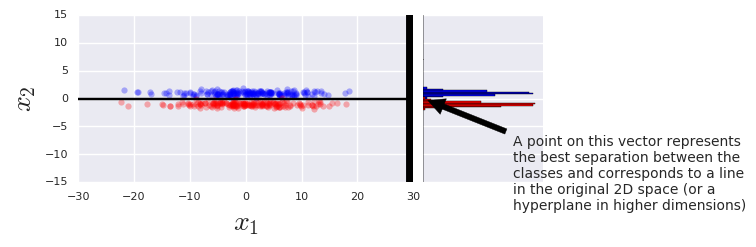
\includegraphics[width=15cm]{best_projection}
\caption{Example of a projection that does discriminate between the data classes}\label{fig:best_proj}
\end{figure}

%Asside: In this case, with $\mathbf{w}$ the optimal projection vector for maximally separating the class, we would project $\mathbf{x}$ onto $\mathbf{w}$ y = $\mathbf{w}^Tx$, and make a classification decision based on $y \geq w_o$. You would use Decision theory to decide on $w_o$ that minimises the misclassification rate.

% [PP: A lot of important information are put in the footnote. This suggests either students should know stuff or you think are obvious. I found many of those not to be obvious and very intellectually intimidating. How is it obvious $rank(S_B) \leq K-1$ as $S_B$ is the sum of $K$ matrices that have rank one or less? I would like these notes to be self contained and understood rather than challenging and needing to read more.
%
% Moreover, the whole mathematical argument, suggests that WSW is a projection It is not obvious to me that W is a projection and we to exaplin the meaning of WSW as a projection. The J(W) is not clearly explained.
%
% So we project the class means into a subspace. I do not have the figures here so I am not sure how this works. You say projecting the class means to a subspace. I assume W defines the lines that minimizes the missclassification rate if we use Bayes classifier. I do not see how we project the means to something. Must be obvious but I am missing it.
%
%
% ]

\section{Notes}
\begin{enumerate}
  \item LDA/QDA classifies a new datapoint to the class with the closest centroid. Here `closest' is measured in the Mahalanobis metric, using a pooled covariance estimate.
  \item Under the assumption that the data are multi-variate Gaussian within each class, LDA is a Bayes' classifier (i.e. it minimises the probability of making a mis-classification).
  \item LDA results in linear decision boundaries.
  \item In many cases, when linear decision boundaries are inadequate for separating the classes, QDA can be used, with the cost of needing to estimating more parameters.
  \item LDA needs to approximate the following ($K + K + P^2$) statistics from the data:
  \begin{enumerate}
    \item K priors: $\hat\pi_k = \frac{N_k}{N}$
    \item K means: $\hat\mu_k = \sum_{i \in k} \frac{x_i}{N_k}$
    \item 1 covariance matrix: $\hat\Sigma = \sum_{k=1}^K\sum_{i \in k} \frac{(x_i - \hat\mu_k)(x_i - \hat\mu_k)^T}{N-K}$
  \end{enumerate}
  \item QDA needs to approximate the following ($K + K + K \times P^2$) statistics from the data (notice the possibility for overfitting your training data here):
  \begin{enumerate}
    \item K priors: $\hat\pi_k = \frac{N_k}{N}$
    \item K means: $\hat\mu_k = \sum_{i \in k} \frac{x_i}{N_k}$
    \item K covariance matrices: $\hat\Sigma_k = \sum_{i \in k} \frac{(x_i - \hat\mu_k)(x_i - \hat\mu_k)^T}{N_k}$
  \end{enumerate}
\end{enumerate}

Other interesting and worthwhile references are: \cite{turk1991face}, \cite{belhumeur1997eigenfaces}, \cite{martinez2001pca}.

\bibliography{section_6}
\bibliographystyle{ieeetr}

\end{document}
